\documentclass[journal]{IEEEtran}
\usepackage[a5paper, margin=10mm, onecolumn]{geometry}
\usepackage{tfrupee} % Include tfrupee package
\usepackage{cite}
\usepackage{amsmath,amssymb,amsfonts,amsthm}
\usepackage{algorithmic}
\usepackage{graphicx}
\usepackage{textcomp}
\usepackage{xcolor}
\usepackage{txfonts}
\usepackage{enumitem}
\usepackage{mathtools}
\usepackage{gensymb}
\usepackage{comment}
\usepackage[breaklinks=true]{hyperref}
\usepackage{tkz-euclide} 
\usepackage[latin1]{inputenc}                                
\usepackage{color}                                            
\usepackage{array}                                            
\usepackage{longtable}                                       
\usepackage{calc}                                             
\usepackage{multirow}                                         
\usepackage{hhline}                                           
\usepackage{ifthen}                                           
\usepackage{lscape}

\setlength{\headheight}{1cm} % Set the height of the header box
\setlength{\headsep}{0mm}     % Set the distance between the header box and the top of the text

\begin{document}

\bibliographystyle{IEEEtran}
\renewcommand{\thefigure}{\theenumi}
\renewcommand{\thetable}{\theenumi}
\setlength{\intextsep}{10pt} % Space between text and floats
\numberwithin{equation}{enumi}
\numberwithin{figure}{enumi}
\title{4-4.2-21}
\author{AI24BTECH11016-Jakkula Adishesh Balaji}
\maketitle

\section*{\textbf{Linear Forms (Parameters)}}
\parindent 0pt
Question: \\
\textbf{4.2.21} Find the direction and normal vectors of the line \( F = \frac{9}{5}C + 32 \).

\begin{table}[h!]    	
    \centering
    \begin{tabular}[12pt]{ |c| c|}
    \hline
    Parameter & Description\\ 
    \hline
    $P$ & $\myvec{2\\-3}$ \\
    \hline 
    $Q$ & $\myvec{10\\y}$ \\
    \hline
    $D$ & $Q-P$\\
    \hline 
    Distance & $10$ \\
    \hline
    \end{tabular}

    \caption{Variables Used}
    \label{tab1-1.9-6}
\end{table}

\solution
The normal vector can be found as follows:
\begin{align}
    F - \frac{9}{5}C &= 32 \\
    \begin{pmatrix} 1 & -\frac{9}{5} \end{pmatrix} \begin{pmatrix} F \\ C \end{pmatrix} &= \begin{pmatrix} 32 \\ 0 \end{pmatrix} \\
    \begin{pmatrix} 1 & -\frac{9}{5} \end{pmatrix} x &= 32 \\
    \vec{n}^\top \vec{x} &= 32\\
    \vec{n} &= \begin{pmatrix} 1 \\ -\frac{9}{5} \end{pmatrix}
\end{align}

The direction vector can be found as follows:
\begin{align}
    F &= F \\
    C &= \frac{5}{9}F - \frac{160}{9} \\
    \begin{pmatrix} F \\ C \end{pmatrix} &= F \begin{pmatrix} 1 \\ \frac{5}{9} \end{pmatrix} + \begin{pmatrix} 0 \\ -\frac{160}{9} \end{pmatrix} \\
    \vec{x} &= k \vec{m} + \vec{h} \\
    \vec{m} &= \begin{pmatrix} 1 \\ \frac{5}{9} \end{pmatrix}
\end{align}

Direction vector: \( \vec{m} = \begin{pmatrix} 1 \\ \frac{5}{9} \end{pmatrix} \\
\text{Normal vector: } \vec{n} = \begin{pmatrix} 1 \\ -\frac{9}{5} \end{pmatrix} \)

\begin{figure}[h!]
    \centering
    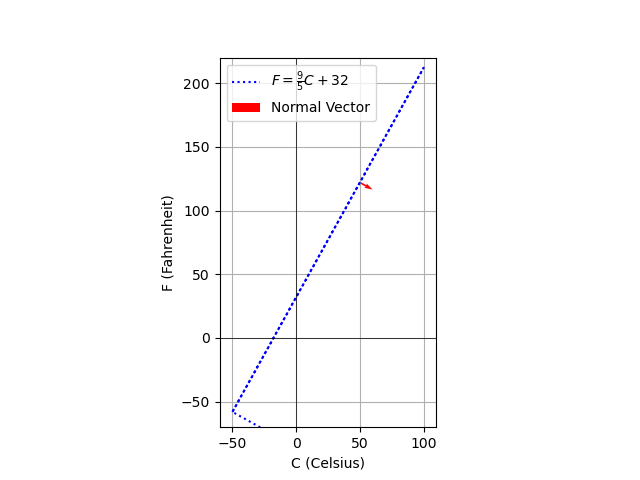
\includegraphics[width = 1\linewidth]{figs/fig.png}
    \caption{Graphical representation of the vectors.}
    \label{stemplot}
\end{figure}

\end{document}

